\subsection{\secState{R}Architecture}\label{s:RuleEngineArchitecture}

\paragraph{Purpose:} The \emph{core process} of \emph{Avoidance Grid Run} (sec. \ref{s:aviudabceGridRun}) and \emph{Mission Control Run} (sec. \ref{s:missionControlRun}) needs to be enhanced based on  the situation. The architecture is based on \emph{aspect-oriented approach} \cite{hill2003jess}. The key ideas and concepts are taken from rule engine implementation for multiagent  navigation system \cite{seyboth2013event}.

\begin{figure}[H]
    \centering
    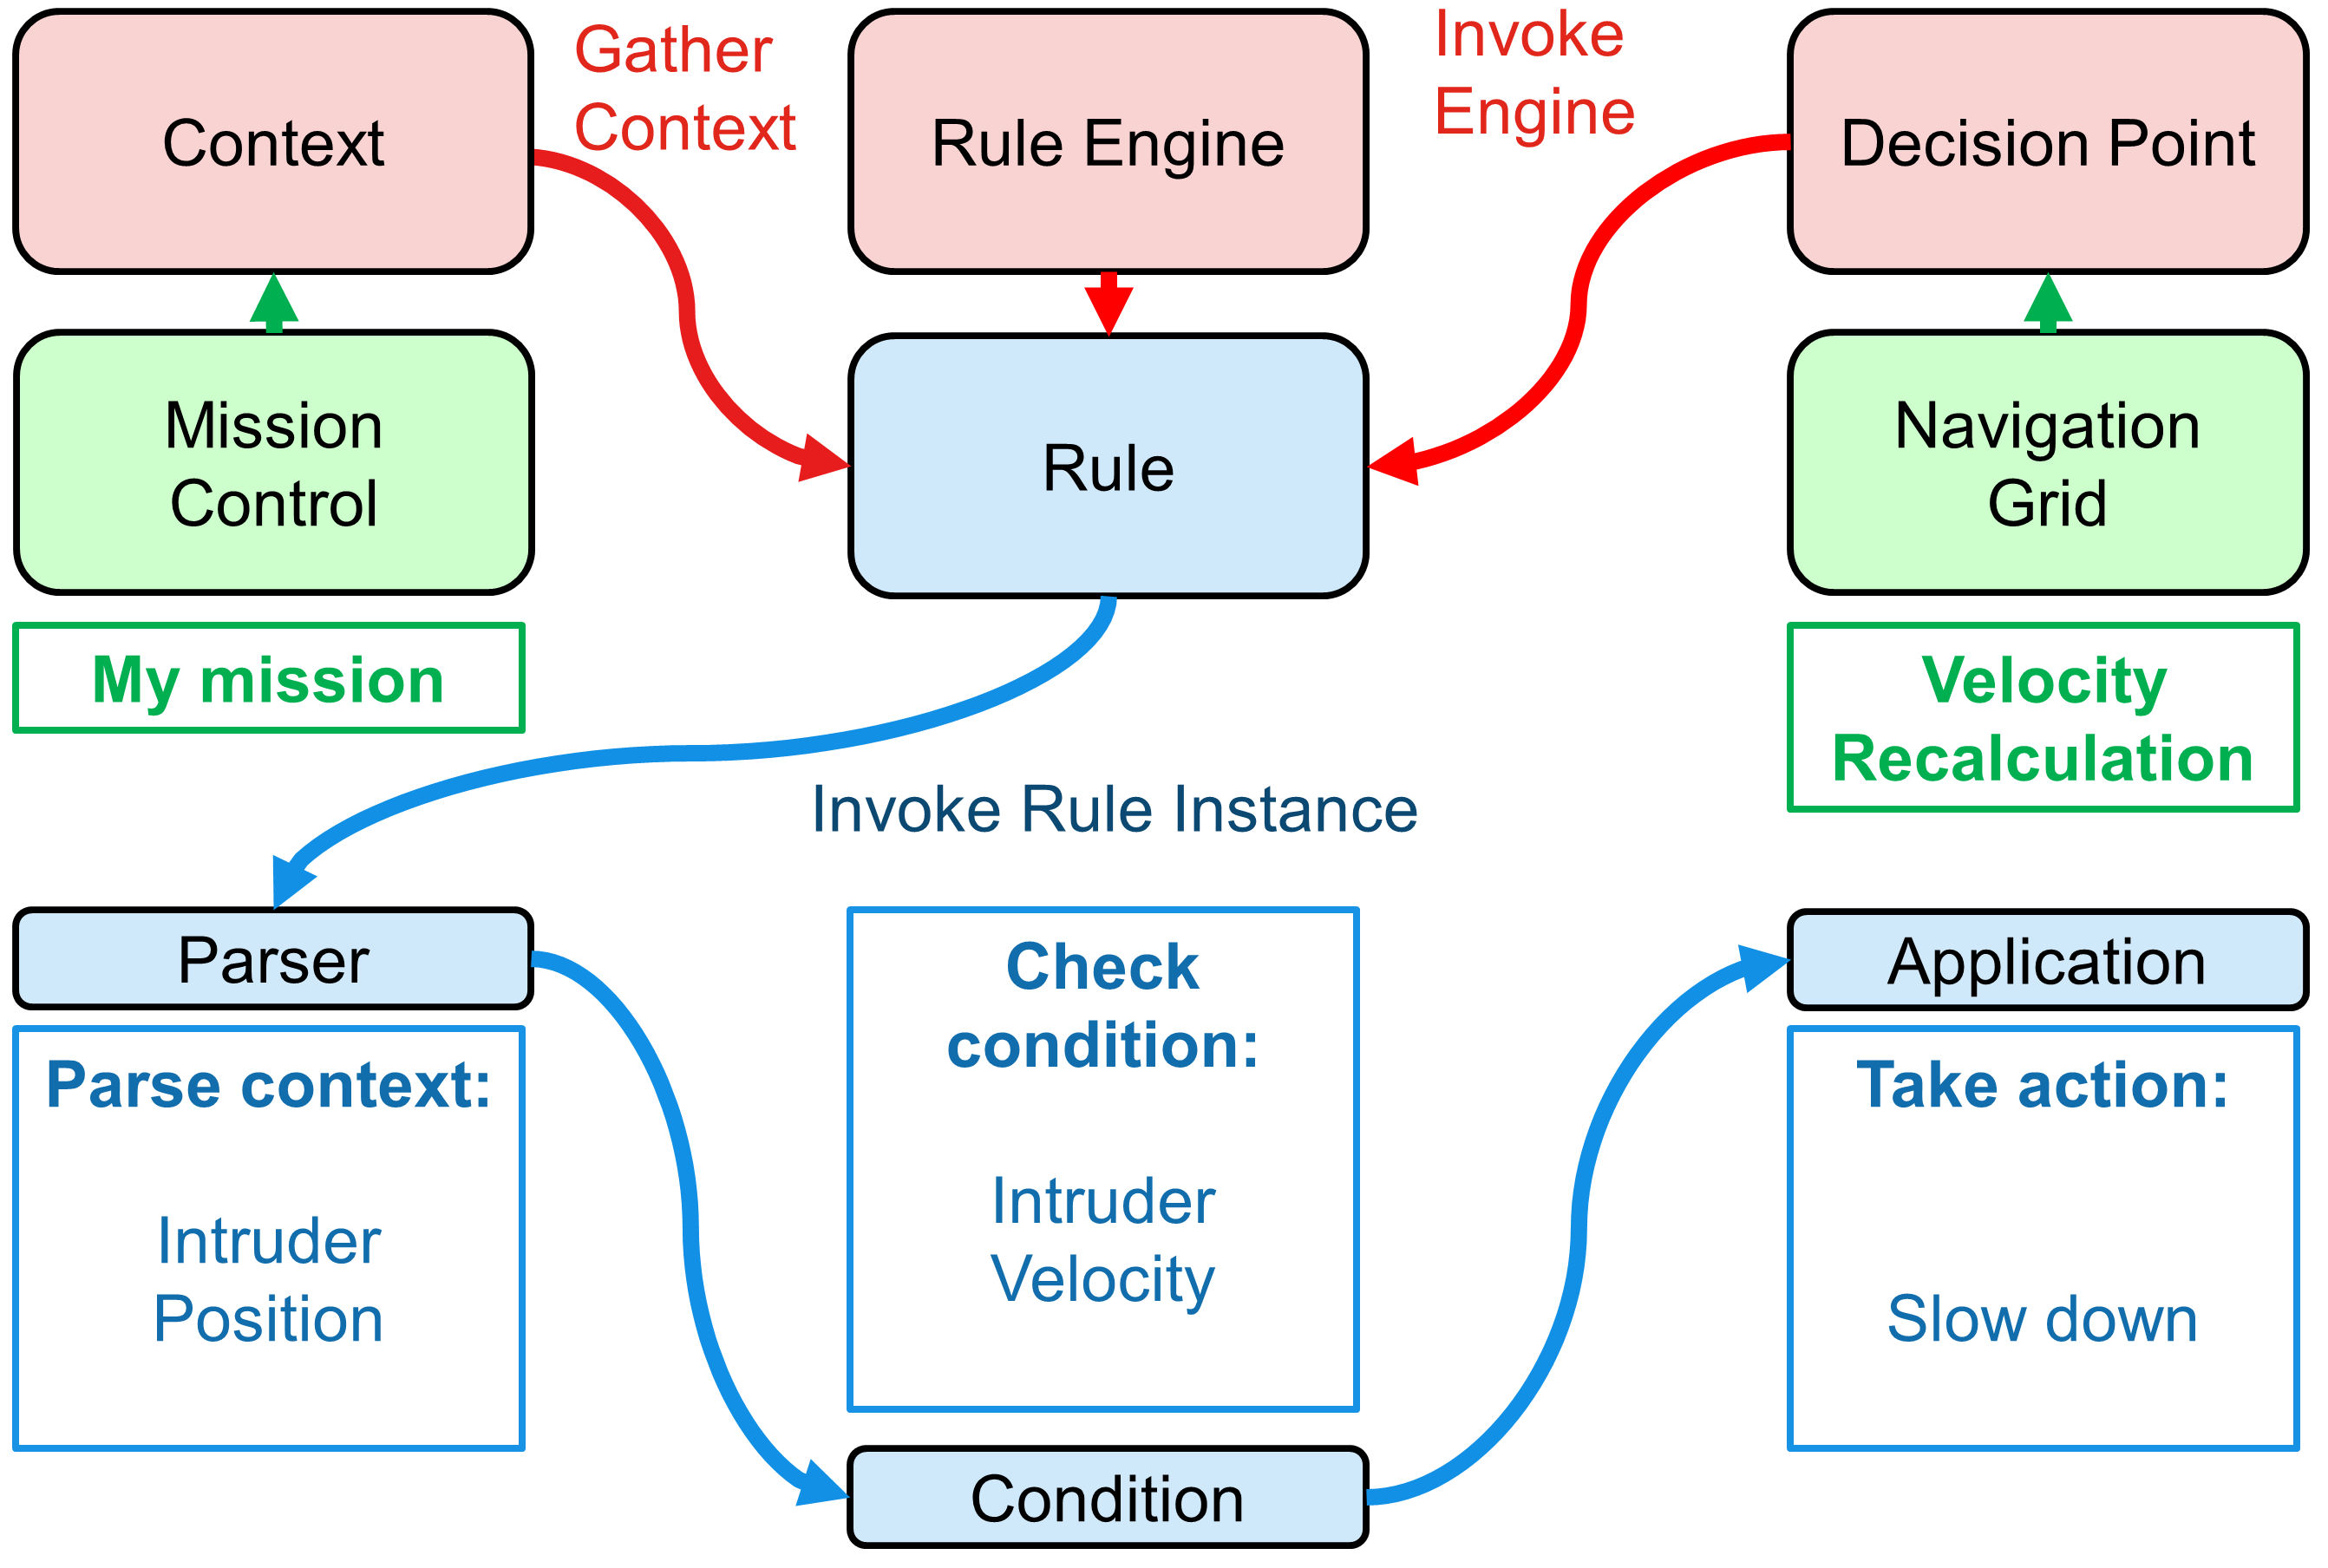
\includegraphics[width=0.7\linewidth]{\FIGDIR/RE013RuleEngineBasicArchitecture}
    \caption{Rule engine components overview.}
    \label{fig:RuleEngineBasicArchitecture}
\end{figure}

\paragraph{Rule Engine:} The program module to inject and run \emph{rules} modifying standard work-flow based on  triggering events. The \emph{aspect-oriented} approach enables to configure rules in \emph{run-time} via predefined process hooks - \emph{Decision Points}. 

\noindent A rules the in context of this work are pieces of code which have a semi-static structure consisting of following parts (fig. \ref{fig:RuleEngineBasicArchitecture}):

\begin{enumerate}
    \item \emph{Decision Point} - hook point in the process where the rule can be attached/detached. If more than one rule is hooked the priority of execution needs to be defined. 
    
    \item \emph{Context} - the \emph{run time context} in a time of \emph{invocation} in our case the \emph{copy} of \emph{Mission Control}, \emph{Avoidance/Navigation Grid} and,  \emph{Collision Cases}.
    
    \item \emph{Parser Method} - optional helper method to parse interesting data set from \emph{Context}. The \emph{parsed data} have better readability.
    
    \item \emph{Condition Check Method} - implementation of the trigger. If the sufficient condition is met, the rule body is applied.
    
    \item \emph{Rule application} - calculations and data structure changes. Mainly, by  \emph{disabling trajectories} in \emph{Reach Set} in our implementation.     
\end{enumerate}

\paragraph{Example:} The \emph{UAS} is flying in controlled airspace.  The \emph{intruder} shows in front of \emph{UAS}. The \emph{UAS} is faster than an \emph{intruder}. The \emph{UAS} tries to obtain permission for \emph{Overtake}. The \emph{UTM} does not allow \emph{overtake}, because of \emph{insufficient UAS maneuverability capability}. The \emph{Rule} (fig. \ref{fig:RuleEngineBasicArchitecture}) with:
\begin{enumerate}
    \item \emph{Context} - UAS Mission Control, containing the actual mission goal and UAS IMU parameters. 
    
    \item \emph{Decision Point} (Joint Point) - Navigation grid, containing projected constraints and reach set approximation.
    
    \item \emph{The rule is invoked:}
    \begin{enumerate}[a.]
        \item \emph{The parser} parses the context which is \emph{intruder`s Position Notification} containing its heading and velocity.
        
        \item \emph{The condition} is checked to \emph{relative intruder velocity}. The \emph{evaluation} is positiv, when the UAS is \emph{pursuing the intruder}.
        
        \item \emph{Application} of \emph{Rule} is the last step, in this case, the \emph{UAS} will slow down.
    \end{enumerate}
\end{enumerate}

\paragraph{Configurability:} The \emph{Rule Engine} enables real-time configuration. The \emph{Enabled Rules Table} have been implemented to enforce specific rules in a specific context. 

The \emph{Rules} can be invoked from \emph{Rule Application}; this enables effective rule chaining and piece-wise functionality split. 
